\documentclass[a4paper,oneside,12pt,pdftex]{article}
\usepackage[bahasa]{babel}
\usepackage[top=3cm,left=2.5cm,bottom=3.9cm,right=2.5cm]{geometry}
\usepackage{times}
\usepackage{graphicx}
\usepackage{wrapfig}
\usepackage{subfig}
\usepackage{array}
\usepackage{multirow}
\usepackage{color}
\usepackage{colortbl}
\definecolor{sectioncolor}{rgb}{0.211764706,0.37254902,0.568627451}
\definecolor{subsectioncolor}{rgb}{0.309803922,0.505882353,0.741176471}
\usepackage{hyperref}
\hypersetup{colorlinks,citecolor=blue,filecolor=black,linkcolor=blue,urlcolor=blue,breaklinks=true}
\usepackage{fancyhdr}
\pagestyle{fancy}
\fancyhead{}
\fancyfoot{}
\lfoot
{
\begin{tabular}{|>{\footnotesize}l|}
\hline
\cellcolor[gray]{0.949019608}Nomor Dokumen: TSTSUB\hspace{1.5cm}Nomor Revisi: 01\hspace{0.7cm}Tanggal: 17/03/10\hspace{1.4cm}Halaman \thepage\hspace{3pt}dari 10\\
\hline
\end{tabular}\\
{\scriptsize\copyright 2010 oleh LSKK STEI-ITB. Pengungkapan dan penggunaan seluruh isi dokumen hanya dapat dilakukan atas ijin tertulis LSKK STEI-ITB Jalan Ganesha 10 Bandung, 40132 Indonesia.}
}
\renewcommand{\headrulewidth}{0pt}


\begin{document}

\addcontentsline{toc}{section}{Lembar Sampul Dokumen}

\begin{wrapfigure}{l}{0.125\textwidth}
\vspace{-0.5cm}

\includegraphics[height=2.6cm]{Ganesha}
%\rule{\linewidth}{0.2mm}
\end{wrapfigure}
\noindent\textbf{\textsf{\LARGE Dokumen Pengembangan Produk}}\\[0.8cm]
\textsf{\large LAB. SISTEM KENDALI \& KOMPUTER, STEI -- ITB}
\rule{\linewidth}{0.2mm}
\vspace{0.5cm}
\begin{center}
\textbf{\textcolor{sectioncolor}{\textsf{\large Lembar Sampul Dokumen}}}\\[1.1cm]
\end{center}

\arrayrulecolor{white}
\setlength\doublerulesep{11pt}

\begin{tabular}{p{4cm}>{\columncolor{backgroundcolor}}p{10.5cm}}
Judul Dokumen & DOKUMEN DESAIN PRODUK:\\[0.1cm]
 & \cellcolor{backgroundcolor}\emph{PUSPA}\\
\hline\hline
\end{tabular}

\begin{tabular}{p{4cm}p{10.5cm}}
Jenis Dokumen & \cellcolor{backgroundcolor}DSG: DESAIN PRODUK\\
 & \hspace{1.25cm}\textmd{\textsf{\scriptsize Catatan: Dokumen ini dikendalikan penyebarannya oleh LSKK, STEI -- ITB}}\\[0.4cm]
\end{tabular}

\begin{tabular}{p{4cm}p{10.5cm}}
Nomor Dokumen & \cellcolor{backgroundcolor}DSG\\
\hline\hline
\end{tabular}

\begin{tabular}{p{4cm}p{10.5cm}}
Nomor Revisi & \cellcolor{backgroundcolor} 02\\
\hline\hline
\end{tabular}

\begin{tabular}{p{4cm}p{10.5cm}}
Nama Berkas & \cellcolor{backgroundcolor}B300.pdf\\
\hline\hline
\end{tabular}

\begin{tabular}{p{4cm}p{10.5cm}}
Tanggal Penerbitan & \cellcolor{backgroundcolor}17 Maret 2010\\
\hline\hline
\end{tabular}

\begin{tabular}{p{4cm}p{10.5cm}}
Unit Penerbit & \cellcolor{backgroundcolor}PUSPA Dev Team\\
\hline\hline
\end{tabular}

\begin{tabular}{p{4cm}p{10.5cm}}
Banyak Halaman & \cellcolor{backgroundcolor}12\\
 & \\[1.1cm]
\end{tabular}

\arrayrulecolor{black}
\setlength\arrayrulewidth{1pt}

\begin{tabular}{|l|l|l|l|l|l|}
\hline
\multicolumn{6}{|l|}{\cellcolor{backgroundcolor}Data Pengusul}\\
\hline
Pengusul & Nama & \multicolumn{2}{l|}{Erik Prabowo} & Jabatan & \textit{Engineer}\\
 & & \multicolumn{2}{l|}{Rio Andita Setiabakti} & & \textit{Engineer}\\
\hline
\multicolumn{2}{|l|}{Tanggal} & \multicolumn{2}{l|}{17 Maret 2010} & Tanda &\\
\multicolumn{2}{|l|}{} & \multicolumn{2}{l|}{} & Tangan &\\
\hline
\multicolumn{2}{|l|}{Lembaga} & \multicolumn{4}{l|}{Rumah Tenda}\\
\multicolumn{2}{|l|}{} & \multicolumn{4}{l|}{Rakreasi}\\
\hline
\multicolumn{2}{|l|}{Alamat} & \multicolumn{4}{l|}{Jln. Ligar Kencana Blok B No. 8 Bandung 40191}\\
\multicolumn{2}{|l|}{} & \multicolumn{4}{l|}{Jln. Tubagus Ismail VIII No. 68 Bandung 40124}\\
\hline
Telepon & {\footnotesize 022-2509262} & Faks & {\footnotesize 022-2509262} & \textit{e-mail} & {\footnotesize\href{mailto:eprabowo@rumahtenda.web.id}{eprabowo@rumahtenda.web.id}}\\
 & {\footnotesize 022-82523428} & & {\footnotesize 022-82523428} & & {\footnotesize\href{mailto:rio.andita@gmail.com}{rio.andita@gmail.com}}\\
\hline
\end{tabular}

\vspace{0.75cm}

\arrayrulecolor{black}
\setlength\arrayrulewidth{0.6pt}

\tableofcontents
\part*{\textcolor{sectioncolor}{\textsf{\large Catatan Sejarah Perbaikan Dokumen}}}
\addcontentsline{toc}{section}{Catatan Sejarah Perbaikan Dokumen}

\begin{tabular}{|p{4cm}|p{11cm}|}
\hline
{\scshape Versi, Tgl, Oleh} & {\scshape Perbaikan}\\
\hline
01, 18 Desember 2009, Erik Prabowo \& Rio Andita Setiabakti & Sebuah dokumen baru yang memaparkan spesifikasi PUSPA.\\
\hline
02, 22 Januari 2010, Erik Prabowo \& Rio Andita Setiabakti & Memperbaharui modul-modul.\\
\hline
03, 17 Maret 2010, Erik Prabowo \& Rio Andita Setiabakti & Memperbaharui setelah mengubah perancangan.\\
\hline
\end{tabular}

\part*{\centering\textsf{\large \textit{TEST} SUBSISTEM PRODUK}}


\section*{\textcolor{sectioncolor}{\textsf{\large PENGANTAR}}}
\addcontentsline{toc}{section}{PENGANTAR}

\subsection*{\textsf{\normalsize 1.1\hspace{0.5cm}RINGKASAN ISI DOKUMEN}}
\addcontentsline{toc}{subsection}{1.1 RINGKASAN ISI DOKUMEN}

Dokumen ini akan memberikan gambaran awal tentang perencanaan pengembangan, analisis pasar, hingga studi kelayakan usaha produksi PUSPA. Kami akan menunjukkan ilustrasi dasar PUSPA berikut konsep rancangannya. Pun dalam dokumen ini kami akan menunjukkan kelayakan usaha produksi PUSPA dengan nilai NPV yang cukup menggiurkan.

\subsection*{\textcolor{subsectioncolor}{\textsf{TUJUAN PENULISAN DAN APLIKASI\slash KEGIATAN}}}
\addcontentsline{toc}{subsection}{TUJUAN PENULISAN DAN APLIKASI\slash KEGIATAN}

Tujuan utama tulisan ini dibuat adalah agar para penulis dokumen ini, yang sedang mengikuti Program Magister Teknik Elektro Opsi Teknologi Media Digital dan Game di ITB, dapat memenuhi salah satu dari persyaratan-persyaratan pembuatan produk yang nantinya akan menjadi bahan tesis.
Tulisan ini ditujukan kepada tim dan pembimbing tesis LSKK STEI--ITB.

Maksud dari penulisan dokumen ini adalah untuk memberikan rincian spesifikasi yang lebih dalam,
yang dari situ akan terlihat lebih jelas juga bagaimana PUSPA dirancang.

\subsection*{\textcolor{subsectioncolor}{\textsf{REFERENSI}}}
\addcontentsline{toc}{subsection}{REFERENSI}
%\begin{itemize}
%\item Han J. Y., \emph{Low-cost multi-touch sensing through frustrated total internal reflection}.\\ 
%  UIST '05: Proceedings of the 18th annual ACM symposium on User Interface Software and Technology, pp. 115-118. ACM, 2005.
%\item Han J. Y., \emph{Multi-touch sensing through frustrated total internal reflection}.\\
%  SIGGRAPH '05: ACM SIGGRAPH 2005 Sketches, pp. 145. ACM, 2005.
%\item Jurafsky D. \& Martin J. H., \emph{Speech and Language Processing}, 2nd ed.\\
%  Upper Saddle River, New Jersey 07458: Pearson Education, Inc., 2009.
%\item Nakatani L. H. \& Rohrlich J. A., \emph{Soft machines: A philosophy of user-computer interface design}.
%  CHI '83: Proceedings of the SIGCHI conference on Human Factors in Computing Systems, pp. 19-23. ACM, 1983.
%\item Poslad S., \emph{Ubiquitous Computing: Smart Devices, Environments and Interactions}.\\
%  Wiley \& Sons, Gebundene Ausgabe, 2009.
%\item Thalmann D., Noser H. \& Huang Z., \emph{Autonomous Virtual Actors Based on Virtual Sensors}, \emph{Creating Personalities for Synthetic Actors}, pp. 25-42, 1997.
%\item Trappl R. \& Petta P. (Eds.), \emph{Creating Personalities for Synthetic Actors: Towards Autonomous Personality Agents}, Vol. 1195. Springer, 1997.
%\item Walker M. A. \& Rambow O., \emph{Computer Speech and Language, Special Issue on Spoken Language Generation}, July 2002.
%\item Wilson A. D., \emph{TouchLight: an imaging touch screen and display for gesture-based interaction}.
%  ICMI '04: Proceedings of the 6th international conference on Multimodal interfaces, pp. 69-76. ACM, 2004.
%\end{itemize}

\subsection*{\textcolor{subsectioncolor}{\textsf{DAFTAR SINGKATAN \& ISTILAH}}}
\addcontentsline{toc}{subsection}{DAFTAR SINGKATAN \& ISTILAH}

\begin{tabular}{|c|c|}
\hline
{\scshape Singkatan} & {\scshape Arti}\\
\hline
3D & 3 Dimensional\\
\hline
CS & ClientSocket (modul)\\
\hline
DM & DialogueManager (modul)\\
\hline
FD & FaceDetector (modul)\\
\hline
GUI & Graphical User Interface\\
\hline
KB & KnowledgeBase (modul)\\
\hline
NLA & NaturalLanguageAnalyser (modul)\\
\hline
NLG & NaturalLanguageGenerator (modul)\\
\hline
NLP & Natural Language Processing\\
\hline
PUSPA & {\scshape Puspa}'s an Understanding Synthespian that Provides Assistance\\
\hline
SR & SpeechRecogniser (modul)\\
\hline
SS & ServerSocket (modul)\\
\hline
SS & SpeechSynthesiser (modul)\\
\hline
ST & Synthespian (modul)\\
\hline
STT & Speech-To-Text\\
\hline
Surel & Surat elektronik\\
\hline
Synthespian & Synthetic thespian\\
\hline
TM & TaskManager (modul)\\
\hline
TTS & Text-To-Speech\\
\hline
UI & UserInterface (modul)\\
\hline
\end{tabular}



\section*{\textcolor{sectioncolor}{\textsf{\large HST: \textit{HW SUBSYSTEM TEST SPECIFICATION}}}}
\addcontentsline{toc}{section}{HST: \textit{HW SUBSYSTEM TEST SPECIFICATION}}

\subsection*{\textcolor{subsectioncolor}{\textsf{1. \textit{SCOPE}}}}
\addcontentsline{toc}{subsection}{1. \textit{SCOPE}}

\subsection*{\textcolor{subsectioncolor}{\textsf{2. KONFIGURASI \textit{TEST}}}}
\addcontentsline{toc}{subsection}{2. KONFIGURASI \textit{TEST}}

\subsection*{\textcolor{subsectioncolor}{\textsf{3. SYARAT-SYARAT \textit{TEST}}}}
\addcontentsline{toc}{subsection}{3. SYARAT-SYARAT \textit{TEST}}

\subsection*{\textcolor{subsectioncolor}{\textsf{4. \textit{TEST PROCEDURES}}}}
\addcontentsline{toc}{subsection}{4. \textit{TEST PROCEDURES}}

\subsection*{\textcolor{subsectioncolor}{\textsf{5. \textit{TEST RESULT}}}}
\addcontentsline{toc}{subsection}{5. \textit{TEST RESULT}}



\section*{\textcolor{sectioncolor}{\textsf{\large SST: \textit{SW SUBSYSTEM TEST SPECIFICATION}}}}
\addcontentsline{toc}{section}{SST: \textit{SW SUBSYSTEM TEST SPECIFICATION}}

\subsection*{\textcolor{subsectioncolor}{\textsf{1. \textit{SCOPE}}}}
\addcontentsline{toc}{subsection}{1. \textit{SCOPE}}

\subsubsection*{\textit{Server}}
Lingkup fungsional subsistem \textit{server} mencakup:
\begin{enumerate}
\item membuka layanan TCP/IP pada \textit{port} tertentu, dan menyiapkan diri untuk menerima masukan yang dikirim oleh subsistem \textit{client},
%\item menganalisa susunan karakter-karakter UTF-8 menjadi bentuk perwakilan yang dimengerti oleh sistem,
\item mengolah masukan bentuk perwakilan tersebut untuk menghasilkan tanggapan yang akan membuat hubungan masukan dan keluarannya menjadi seperti percakapan,
\item memenuhi prasyarat-prasyarat pelaksanaan tugas apabila terdapat unsur permintaan dalam masukan yang diberikan oleh pengguna,
%\item menghasilkan tanggapan sehingga menjadi bentuk yang dimengerti pengguna,
\item dan mengirimkan keluarannya ke subsistem \textit{client}.
\end{enumerate}
Lingkup kinerja subsistem \textit{server} mencakup:
\begin{enumerate}
\item keluwesan komunikasi dengan subsistem \textit{client}, %lebih daripada satu,
%\item kemapanan dan ketepatan dalam menganalisa masukan,
\item dan baiknya penerapan algoritma dalam menyimulasikan percakapan.
%\item terlaksananya tugas yang diberikan,
%\item dan mutu dari hasil akhir yang dikeluarkan.
\end{enumerate}
Lingkup perancangan subsistem \textit{server} mencakup:
\begin{enumerate}
\item penentuan algoritma yang berpengaruh pada ciri-ciri percakapan yang disimulasikan,
\item dan penentuan arsitektur agen percakapan yang diterapkan.
\end{enumerate}

\subsubsection*{\textit{Client}}
Lingkup fungsional subsistem \textit{client} mencakup:
\begin{enumerate}
\item membentuk sambungan dengan subsistem \textit{server},
\item menyiapkan diri untuk mendengarkan apa yang mungkin akan diucapkan oleh pengguna,
%\item menampilkan wajah PUSPA,
%\item mengenali pengguna,
\item mengirimkan apa yang diucapkan oleh pengguna dalam bentuk karakter-karakter UTF-8 ke subsistem \textit{server},
\item menerima karakter-karakter UTF-8 yang dikembalikan oleh subsistem,
\item mengeluarkan suara pengucapan dari susunan karakter-karakter tersebut,
\item dan menampilkan sejarah percakapan.
%\item dan melakukan animasi yang menyimulasikan gerakan wajah manusia.
\end{enumerate}
Lingkup kinerja subsistem \textit{client} mencakup:
\begin{enumerate}
\item keluwesan komunikasi dengan subsistem \textit{server},
%\item baiknya pengenalan wajah pengguna,
\item baiknya pengenalan ucapan pengguna,
\item dan kejelasan pengucapan teks.
%\item dan kemiripan penggambaran gerakan wajah.
\end{enumerate}
Lingkup perancangan subsistem \textit{client} mencakup:
\begin{enumerate}
\item pemilihan alat pendukung yang mempengaruhi perancangan sistem secara keseluruhan.
\end{enumerate}

\subsection*{\textcolor{subsectioncolor}{\textsf{2. KONFIGURASI \textit{TEST}}}}
\addcontentsline{toc}{subsection}{2. KONFIGURASI \textit{TEST}}

\subsubsection*{\textit{Server}}
Konfigurasi pada \textit{server} yang telah diketahui jalan mencakup:
\begin{itemize}
\item direktori \texttt{common} dikerahkan ke peubah \texttt{COMMONDIR},
\item peubah tersebut dikerahkan ke peubah \texttt{VPATH} pada Makefile,
\item peubah tersebut disertakan, dengan \textit{flag} \verb!-I$(COMMONDIR)!
\item direktori \textit{header} Python disertakan, dengan \textit{flag} \texttt{-I/usr/include/python2.5},
\item semua bentuk penyertaan di atas dikerahkan pada peubah \texttt{CXXFLAGS},
\item PCRE di-\textit{link} dengan \textit{flag} \texttt{-lpcrecpp},
\item Python di-\textit{link} dengan \textit{flag} \texttt{-lpython2.5},
\item semua bentuk \textit{link} di atas dikerahkan pada peubah \texttt{LDFLAGS},
\item buat aturan target akhir dengan persyaratan berkas objek tiap berkas kode sumber,
\item buat perintah \verb!$(CXX) $(LDFLAGS) $(OBJECTS) -o puspa! di bawahnya,
\item dan buat aturan untuk berkas objek tiap modul yang mensyaratkan berkas \textit{header}-nya.
\end{itemize}

\subsubsection*{\textit{Client}}
Konfigurasi pada \textit{client} yang telah diketahui jalan mencakup:
\begin{itemize}
\item arsitektur yang digunakan adalah 32/64-bit Universal,
\item SDK dasar yang digunakan adalah SDK Mac OS X 10.5,
\item \textit{framework} OpenGL di-\textit{link},
\item libobj di-\textit{link} dengan \textit{flag} \texttt{-lobj} pada penyetelan ``Other Linker Flags'',
\item direktori \texttt{/usr/local/include} disertakan pada penyetelan ``Header Search Paths'',
\item dan direktori \texttt{/usr/local/lib} disertakan pada penyetelan ``Library Search Paths''.
\end{itemize}

\subsection*{\textcolor{subsectioncolor}{\textsf{3. SYARAT-SYARAT \textit{TEST}}}}
\addcontentsline{toc}{subsection}{3. SYARAT-SYARAT \textit{TEST}}

\subsubsection*{\textit{Server}}
\begin{enumerate}
\item Pustaka Standar C
\item Pustaka POSIX C, terutama Berkeley socket API
\item Pustaka Standar C++
\item PCRE
\item Python/C API
\item NLTK
\end{enumerate}

\subsubsection*{\textit{Client}}
\begin{enumerate}
\item Pustaka Standar C
\item Pustaka POSIX C, terutama Berkeley socket API
\item Pustaka Standar C++
\item Cocoa
\item OpenGL
\item libobj
\end{enumerate}

\subsection*{\textcolor{subsectioncolor}{\textsf{4. \textit{TEST PROCEDURES}}}}
\addcontentsline{toc}{subsection}{4. \textit{TEST PROCEDURES}}


\subsubsection*{\textit{Server}}

Pengujian subsistem ini dilakukan dengan menggunakan subsistem \textit{server} yang sudah mencakup modul ServerSocket dan DialogueManager,
dan dibantu dengan program pengujian modul ClientSocket,
yang berperan sebagai \textit{client} sederhana berbentuk konsol dengan masukan dan keluaran teks.
Gambar \ref{ServerOnServerTest} dan Gambar \ref{ClientOnServerTest} menunjukkan proses pengujian subsistem ini.

\begin{figure}
\centering
\subfloat[\textit{Server}]{\label{ServerOnServerTest}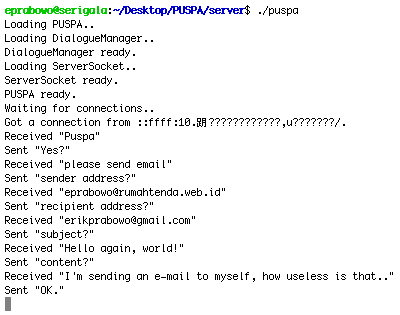
\includegraphics[width=0.5\textwidth]{ServerOnServerTest}}
\subfloat[\textit{Client}]{\label{ClientOnServerTest}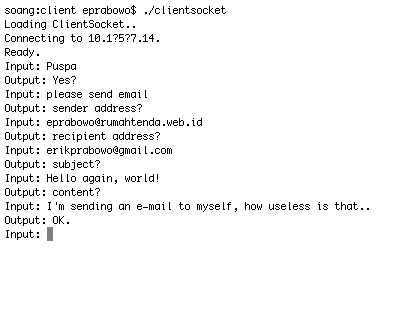
\includegraphics[width=0.5\textwidth]{ClientOnServerTest}}
\caption{Pengujian subsistem \textit{server}}
\label{ServerTest}
\end{figure}


\subsubsection*{\textit{Client}}

Pengujian subsistem ini dilakukan dengan menggunakan subsistem \textit{client} yang sudah mencakup modul ClientSocket, Synthespian, dan UserInterface,
dan dibantu dengan program pengujian modul ServerSocket,
yang berperan sebagai \textit{server} sederhana yang hanya mengembalikan karakter-karakter yang sama dengan masukan yang didapat dari subsistem \textit{client}.
Gambar \ref{ClientOnClientTest} dan Gambar \ref{ServerOnClientTest} menunjukkan proses pengujian subsistem ini.

\begin{figure}
\centering
\subfloat[\textit{Kalimat 1}]{\label{ClientOnClientTest1}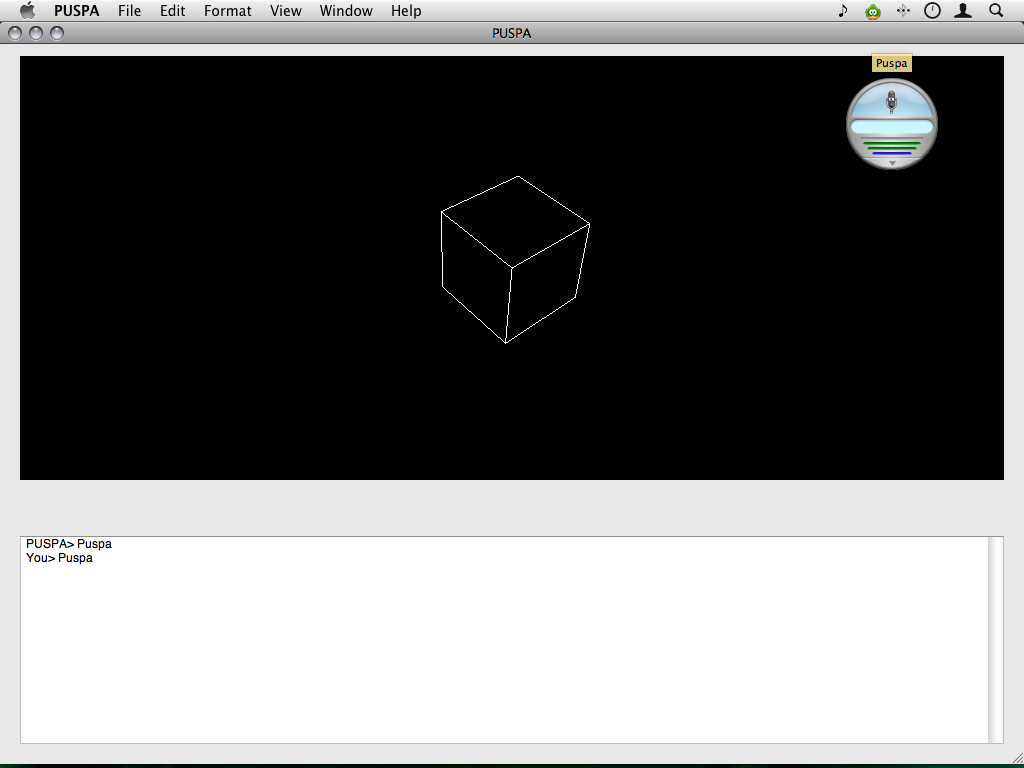
\includegraphics[width=0.5\textwidth]{ClientOnClientTest1}}
\subfloat[\textit{Kalimat 2}]{\label{ClientOnClientTest2}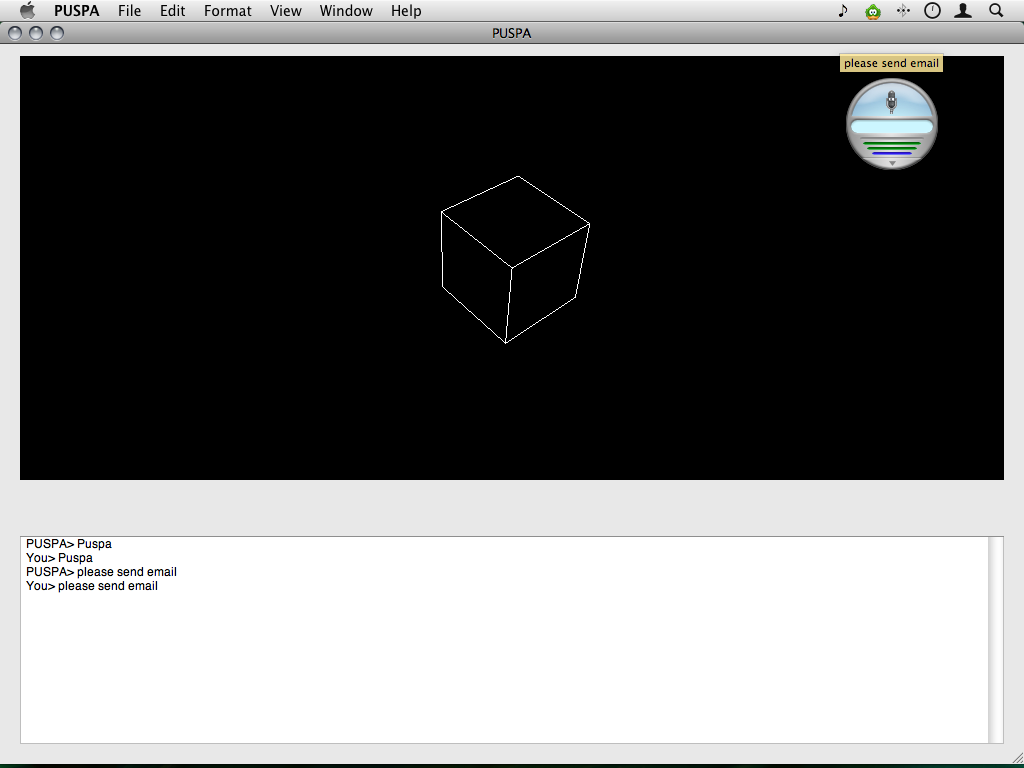
\includegraphics[width=0.5\textwidth]{ClientOnClientTest2}}\\
\subfloat[\textit{Kalimat 3}]{\label{ClientOnClientTest3}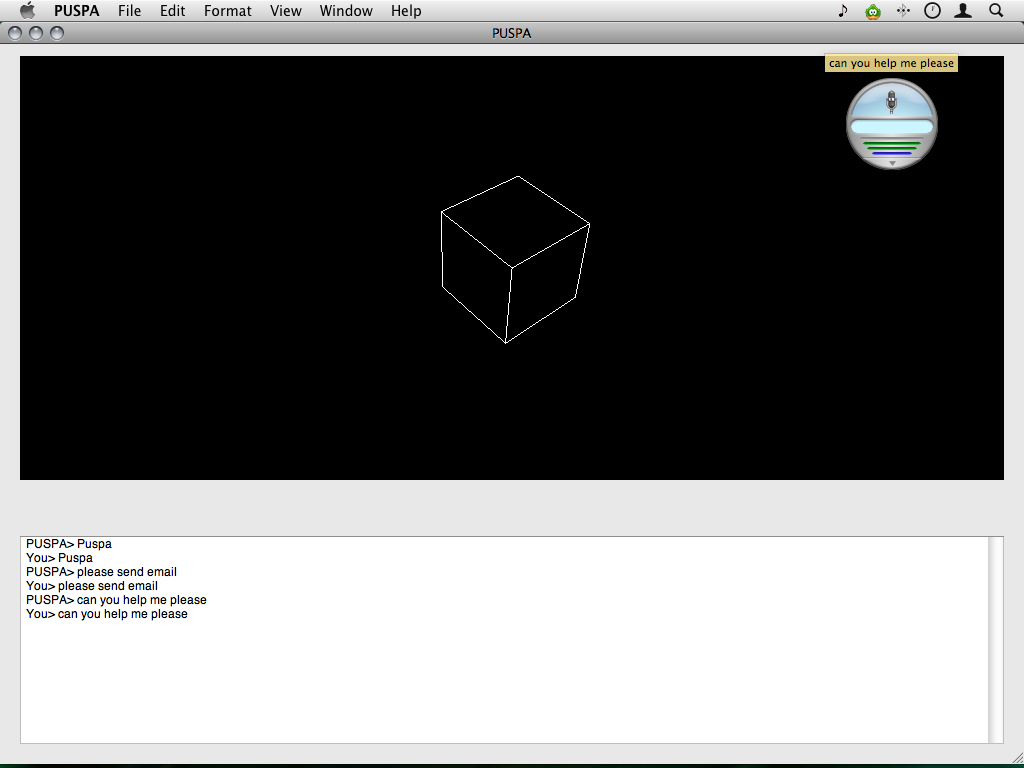
\includegraphics[width=0.5\textwidth]{ClientOnClientTest3}}
\subfloat[\textit{Kalimat 4}]{\label{ClientOnClientTest4}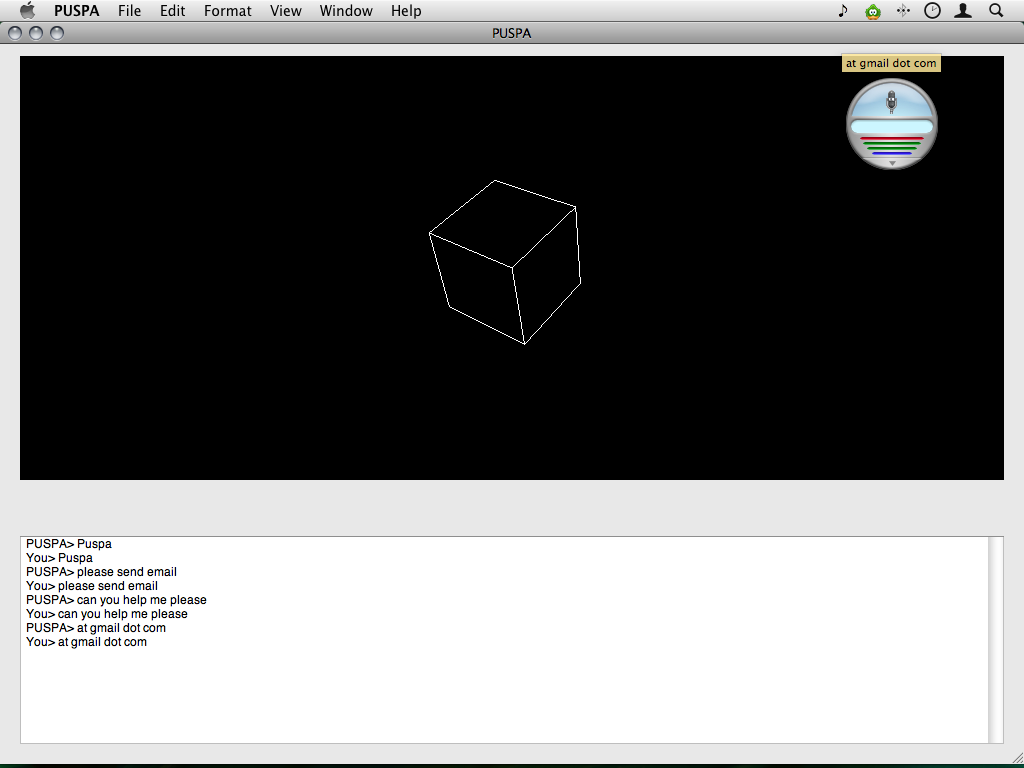
\includegraphics[width=0.5\textwidth]{ClientOnClientTest4}}
\caption{Pengujian subsistem \textit{client}}
\label{ClientOnClientTest}
\end{figure}

\begin{figure}
\centering
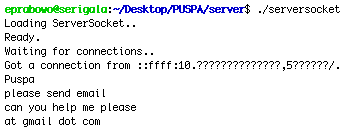
\includegraphics[width=0.5\textwidth]{ServerOnClientTest}
\caption{Yang terjadi pada \textit{server} (sederhana) saat subsistem \textit{client} diuji}
\label{ServerOnClientTest}
\end{figure}

\subsection*{\textcolor{subsectioncolor}{\textsf{5. \textit{TEST RESULT}}}}
\addcontentsline{toc}{subsection}{5. \textit{TEST RESULT}}

\subsubsection*{\textit{Server}}
Hasil pengujian subsistem ini sama seperti gabungan pengujian modul ServerSocket dan DialogueManager.

\subsubsection*{\textit{Client}}
\textit{Tooltip} yang terlihat menunjukkan suara yang dikenali dan diucapkan oleh subsistem ini,
berhubung sudah dilengkapi dengan kemampuan \textit{speech recognition} dan \textit{speech synthesis}.
Gambar yang muncul hanya berupa kubus karena berkas OBJ yang di-\textit{parse} pada modul Synthespian baru gambar kubus,
belum gambar kepala manusia.



\section*{\textcolor{sectioncolor}{\textsf{\large BUG: \textit{BUGS BOOK}}}}
\addcontentsline{toc}{section}{BUG: \textit{BUGS BOOK}}


\section*{\textcolor{sectioncolor}{\textsf{\large ERR: \textit{ERROR REPORT}}}}
\addcontentsline{toc}{section}{ERR: \textit{ERROR REPORT}}


\section*{\textcolor{sectioncolor}{\textsf{\large CHR: \textit{CHANGE REQUESTS}}}}
\addcontentsline{toc}{section}{CHR: \textit{CHANGE REQUESTS}}

\subsection*{\textcolor{subsectioncolor}{\textsf{1. \textit{PREVIOUS VERSION}}}}
\addcontentsline{toc}{subsection}{1. \textit{PREVIOUS VERSION}}

\subsubsection*{Bahasa Alami}
Sebelum pengubahan, bahasa alami utama PUSPA adalah bahasa Indonesia.
Sebab pengubahan dilakukan adalah kenyataan bahwa untuk mengembangkan sistem NLP berbahasa Indonesia,
akan dibutuhkan usaha yang terlalu keras untuk proyek ini,
karena belum cukupnya penerapan NLP berbahasa Indonesia lain yang dapat dijadikan landasan bagi pengembangan PUSPA.

\subsection*{\textcolor{subsectioncolor}{\textsf{2. \textit{CHANGE REQUESTS}}}}
\addcontentsline{toc}{subsection}{2. \textit{CHANGE REQUESTS}}

\subsubsection*{Bahasa Alami}
Diusulkan supaya bahasa alami yang digunakan adalah bahasa Inggris.
Alasan dari usul ini adalah supaya dapat menggunakan sistem NLP berbahasa Inggris yang sudah banyak tersedia,
yang sudah terbukti dapat berjalan dengan betul,
sehingga dapat dijadikan landasan pengembangan PUSPA,
agar pengembangan tersebut tidak usah dilakukan dari dasar.

\subsection*{\textcolor{subsectioncolor}{\textsf{3. \textit{NEW VERSION}}}}
\addcontentsline{toc}{subsection}{3. \textit{NEW VERSION}}
\hyphenation{Speech-Recogniser}

\subsubsection*{Bahasa alami}

Setelah pengubahan, perkembangan berjalan lebih cepat,
karena beberapa modul dapat diterapkan dengan lebih mudah dengan menggunakan sistem yang sudah jadi.
Modul-modul yang sangat terbantu oleh perubahan rancangan ini adalah modul NaturalLanguageAnalyser, modul SpeechRecogniser, dan modul SpeechSynthesiser.

Bagaimanapun, ada beberapa hal yang cukup berdampak pada penerapannya,
karena sistem-sistem lain yang sudah jadi tersebut memiliki spesifikasi yang tidak begitu saling mendukung,
sehingga cara-cara yang tidak begitu konvensional harus dilakukan untuk mengatasi kesulitan ini.
Modul NaturalLanguageAnalyser pada \textit{server} menggunakan NLTK, dan modul SpeechRecogniser dan modul SpeechSynthesiser pada \textit{client} dapat diterapkan dengan mudah pada Cocoa.



\appendix
\addcontentsline{toc}{section}{LAMPIRAN}


\end{document}
